\documentclass[paperwidth=42in,paperheight=47.75in,portrait]{baposter}

\usepackage[font=small,labelfont=bf]{caption} % Required for specifying captions to tables and figures
\usepackage{booktabs} % Horizontal rules in tables
\usepackage{relsize} % Used for making text smaller in some places
\usepackage[sfdefault,light]{roboto}

\graphicspath{{figures/}} % Directory in which figures are stored
\definecolor{bordercol}{RGB}{100,40,40}
\definecolor{boxcolor}{RGB}{255,255,255}
\definecolor{headerfontcol}{RGB}{179,27,27}
\definecolor{graybox}{RGB}{220,220,220}
\definecolor{greenbox}{RGB}{210,245,210}
\definecolor{greenbox_adj}{RGB}{215,235,215}
\definecolor{bluebox}{RGB}{230,245,255}
\definecolor{bluebox_adj}{RGB}{230,240,250}

\begin{document}

\begin{poster}{
    columns=4,
    borderColor=bordercol,headerColorOne=boxcolor,headerColorTwo=boxcolor,headerFontColor=headerfontcol,boxColorOne=boxcolor,
    background=none,boxshade=plain,
    headershape=rectangle,textborder=none,headerborder=none,
    headerfont=\Large\sf\bf,
    grid=false,linewidth=1
}
{}{\sf\bf Long read sequencing and local graph assembly \\ reveal heterogeneity of telomeres} {
    \vspace{.4em} Grigorev K, Foox J, Bezdan D, Butler D, Mason C \\
    {\small Institute for Computational Biomedicine, Weill Cornell Medicine}
}
{
\includegraphics[scale=1.7]{logo.pdf}}


\headerbox{Abstract}{name=abstract,column=0,row=0,span=1,boxColorOne=graybox,headerColorOne=graybox,headerColorTwo=graybox}
{
    Telomeres are regions of repetitive nucleotide sequences capping eukaryotic chromosomes that protect the ends of chromosomes from deterioration.
    Telomeres are known to generally shorten after each cell replication, eventually blocking somatic cell division and preventing genomic instability.
    As such, their length is an important marker in senescence, where it can inversely correlate with a subject’s age, and in cancers, where both
    telomere shortening and unrestricted elongation have been suggested as risk factors.

    Given their length and repetitive nature, telomeric regions cannot be veritably assembled from reads of kilobase-order lengths (Sanger sequencing)
    or sub-1Kbp reads (second-generation sequencing), making telomere resolution a very costly and generally intractable problem.
    Recently, with third-generation technologies like SMRT and nanopore sequencing attaining read lengths on the order of tens and hundreds kilobase
    pairs, with the longest reads reported as 2Mbp, it became possible to routinely read into the telomeric regions and inspect their structure
    and length.

    We describe a framework for extracting telomeric reads from third-generation sequencing experiments and describing their sequence content and
    prevalent motifs. We find that human telomeric sequences exhibit surprising heterogeneity, suggesting the possibility of localization of previously
    reported non-canonical motifs as well as novel sequences.

    We also propose a local graph assembly algorithm capable of describing the haplotypic diversity of telomeres. Given the lower complexity of such
    reads, established methods for long read overlap and assembly that rely on MinHash sketches and minimizers are unsuitable for this problem and fail
    to detect most correct overlaps when compared to the computationally prohibitive, but mathematically correct Smith-Waterman alignment.
    We implement a modified method relying on \textit{unimizers} (minimizers occurring once within a given read) that improves overlaps and reduces
    complexity of the assembly graph, and locally assemble branching telomeric sequences \\ using the computationally efficient \\ A-Bruijn structure.
}


\headerbox{References}{name=references,column=0,below=abstract}
{
    REFS HERE
    \vspace{1in}
%\renewcommand{\section}[2]{\vskip 0.05em} % Get rid of the default "References" section title
%\nocite{*} % Insert publications even if they are not cited in the poster
%
%\bibliographystyle{unsrt}
%\bibliography{sample} % Use sample.bib as the bibliography file
}


\headerbox{Acknowledgements}{name=acknowledgements,column=0,below=references,above=bottom,boxColorOne=graybox,headerColorOne=graybox,headerColorTwo=graybox}
{
    ACKS HERE
}


\headerbox{Background}{name=telomere_sequencing,span=1,column=1,row=0,boxColorOne=graybox,headerColorOne=graybox,headerColorTwo=graybox}
{
    \begin{center}
        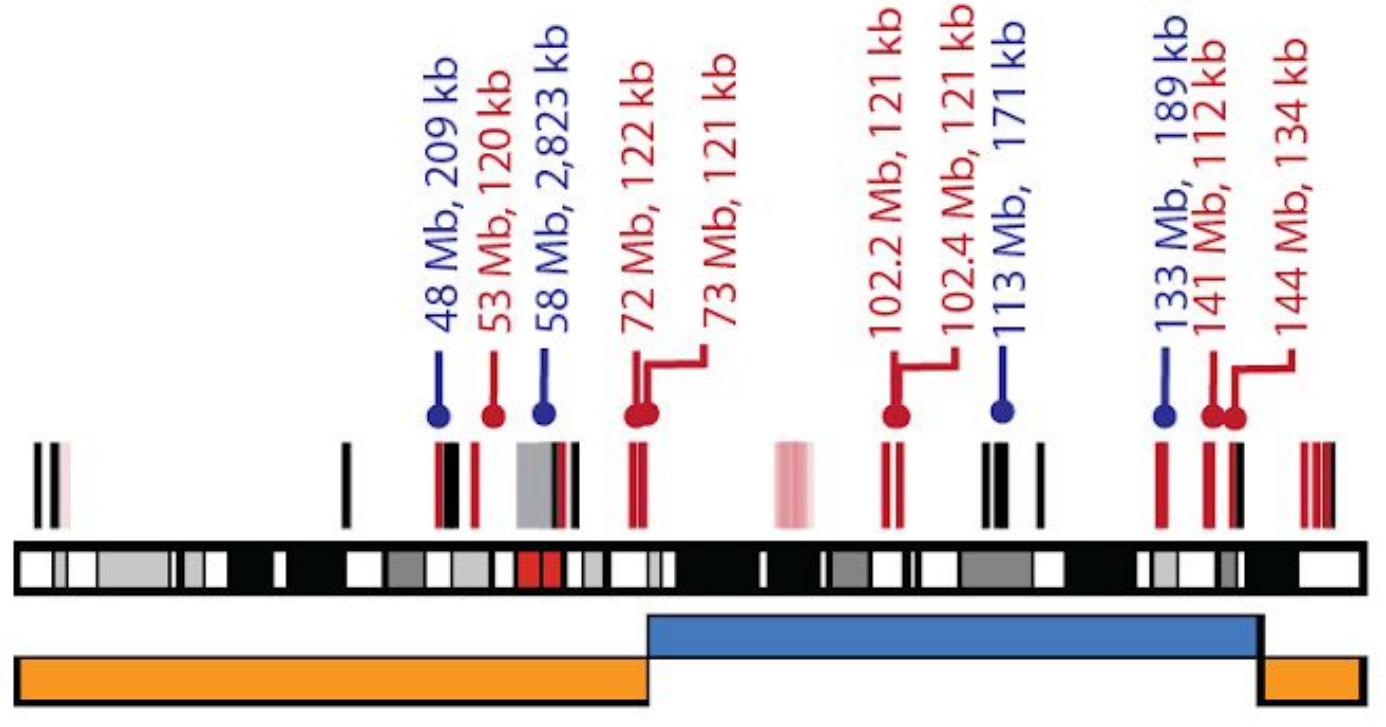
\includegraphics[width=\linewidth]{t2t.png}
            \captionof{figure}{
                Telomere-to-telomere sequencing of the human X chromosome
                    (adapted from \textit{[Miga et al., 2019]}). % 10.1101/735928
            }
    \end{center}
}


\headerbox{}{name=riethman,span=1,column=2,row=0,boxheaderheight=0mm,boxColorOne=graybox,headerColorOne=graybox,headerColorTwo=graybox}
{
    \begin{center}
        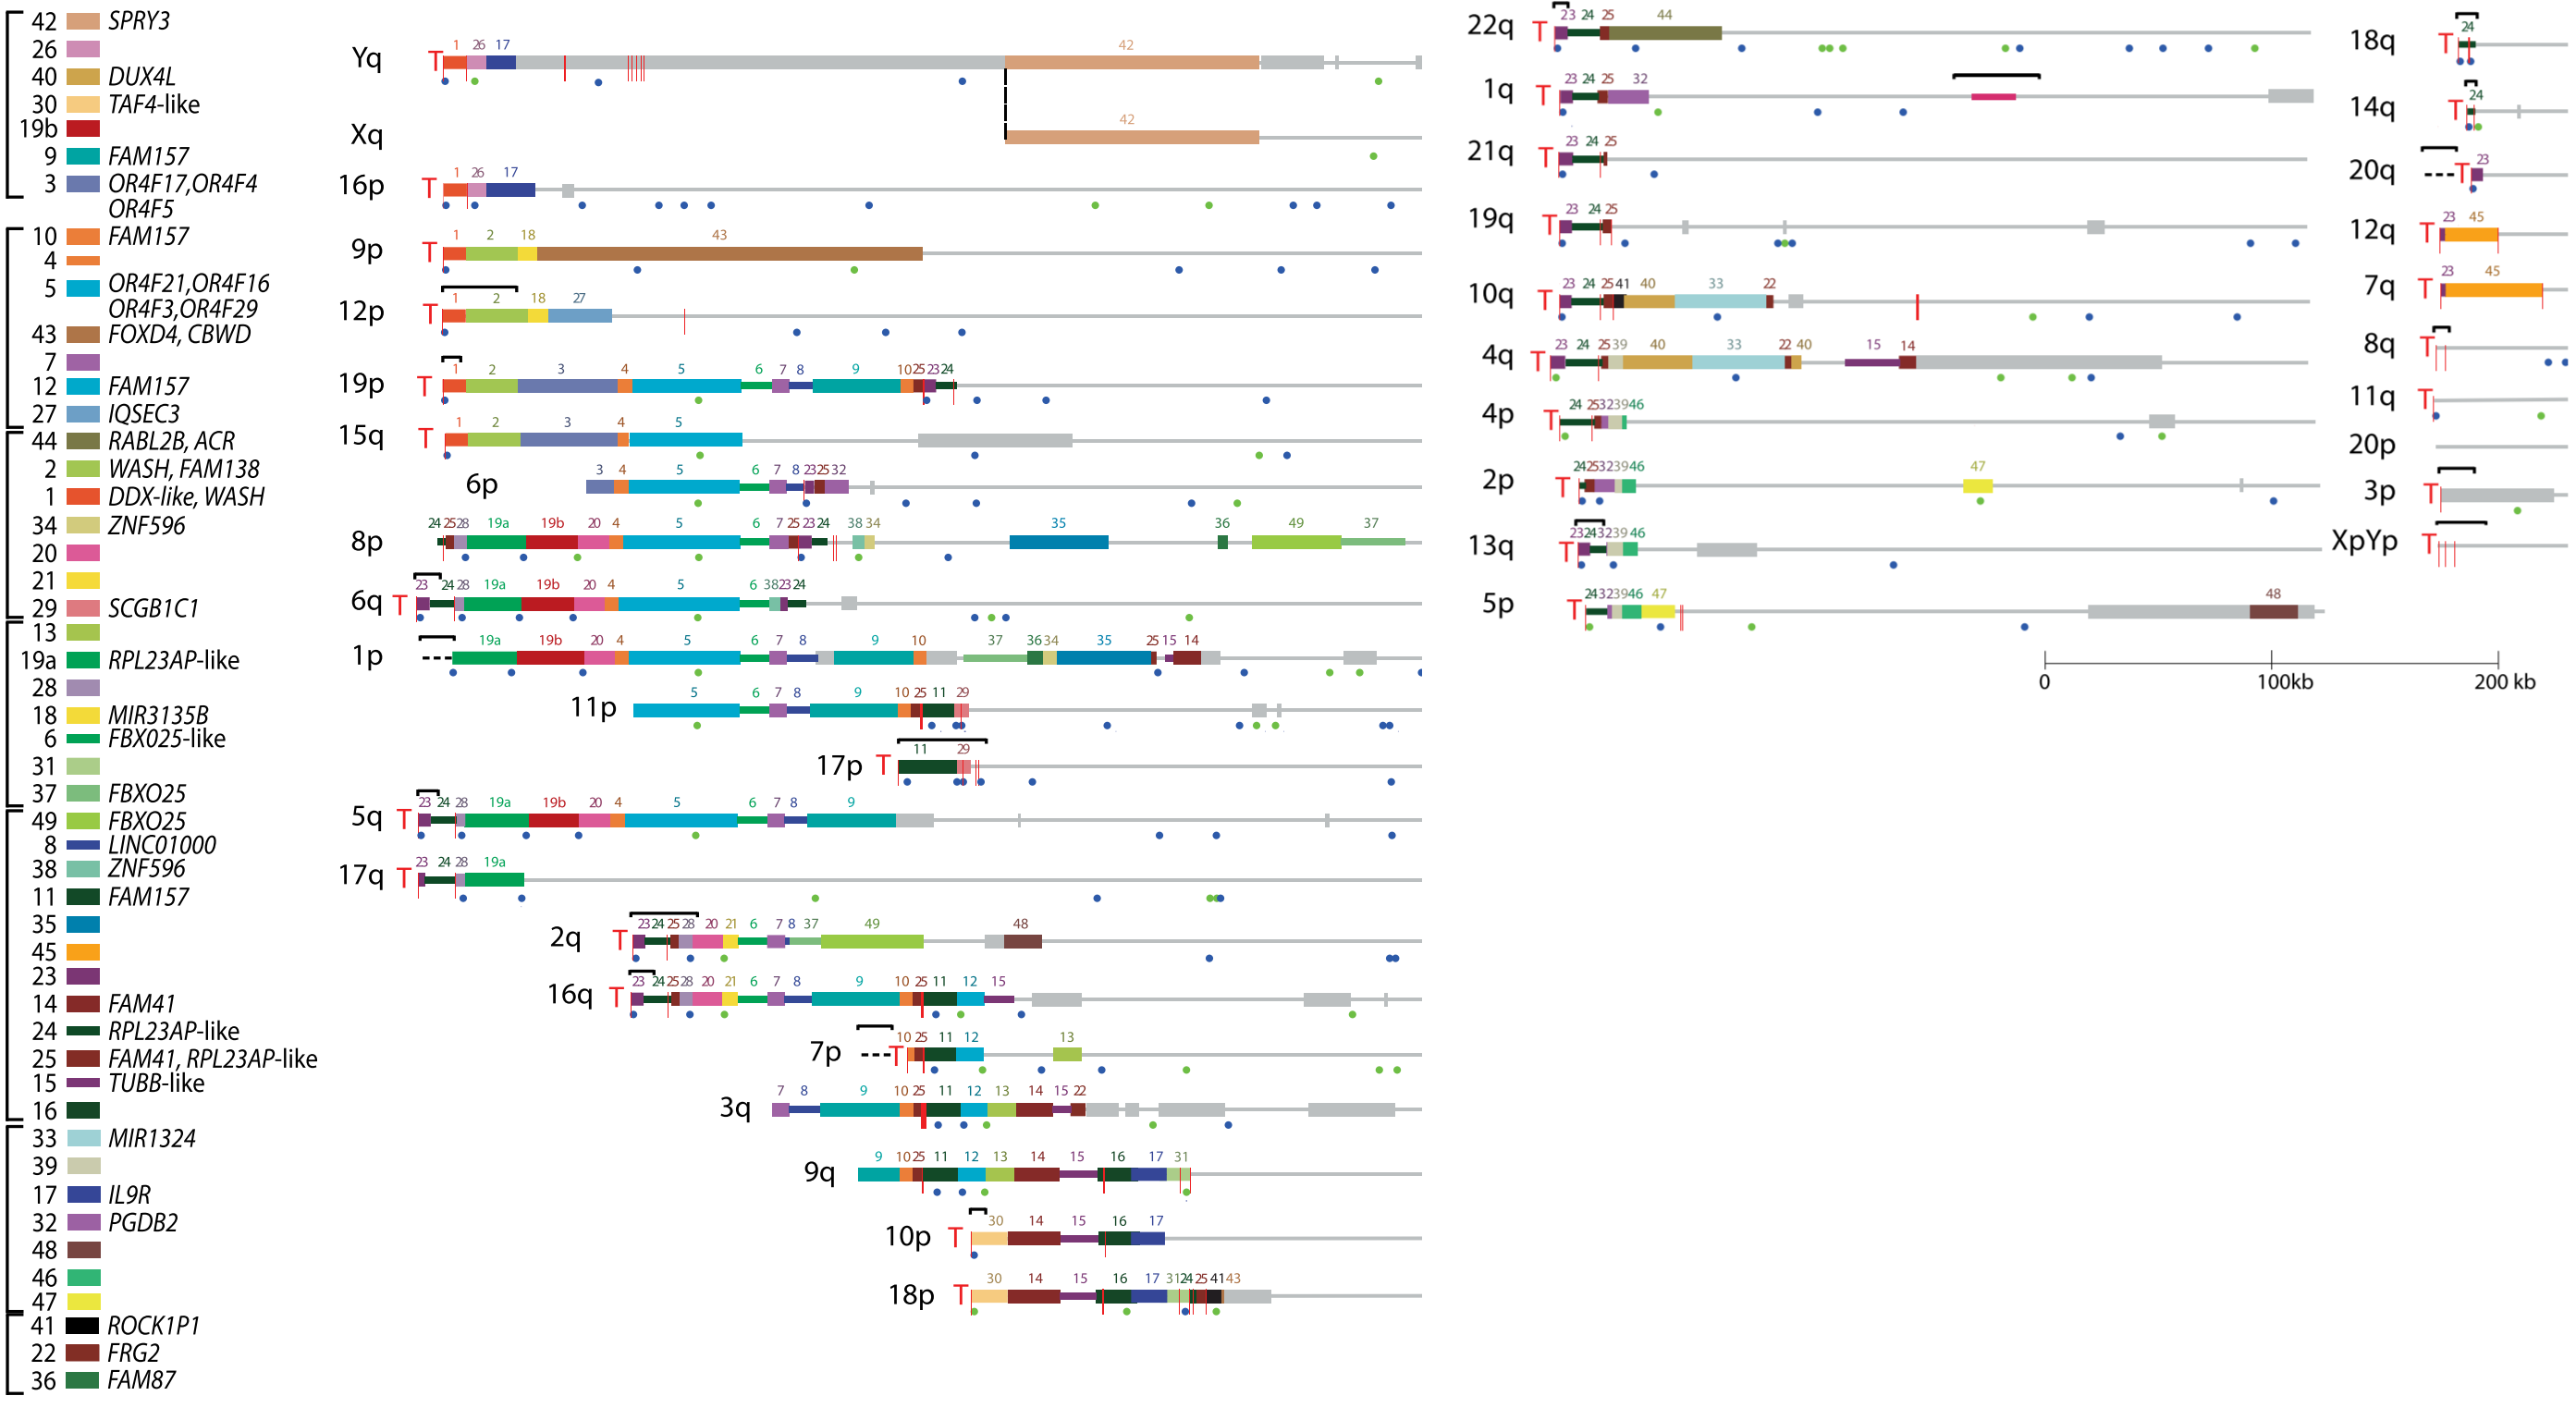
\includegraphics[width=\linewidth]{riethman.png}
            \captionof{figure}{
                Sequencing of the human subtelomeres (adapted from
                \textit{[Stong et al., 2014]}). % 10.1101/gr.166983.113
            }
    \end{center}
}


\headerbox{}{name=wetlab_telomeres,span=1,column=3,row=0,boxheaderheight=0mm,boxColorOne=graybox,headerColorOne=graybox,headerColorTwo=graybox}
{
    \begin{center}
        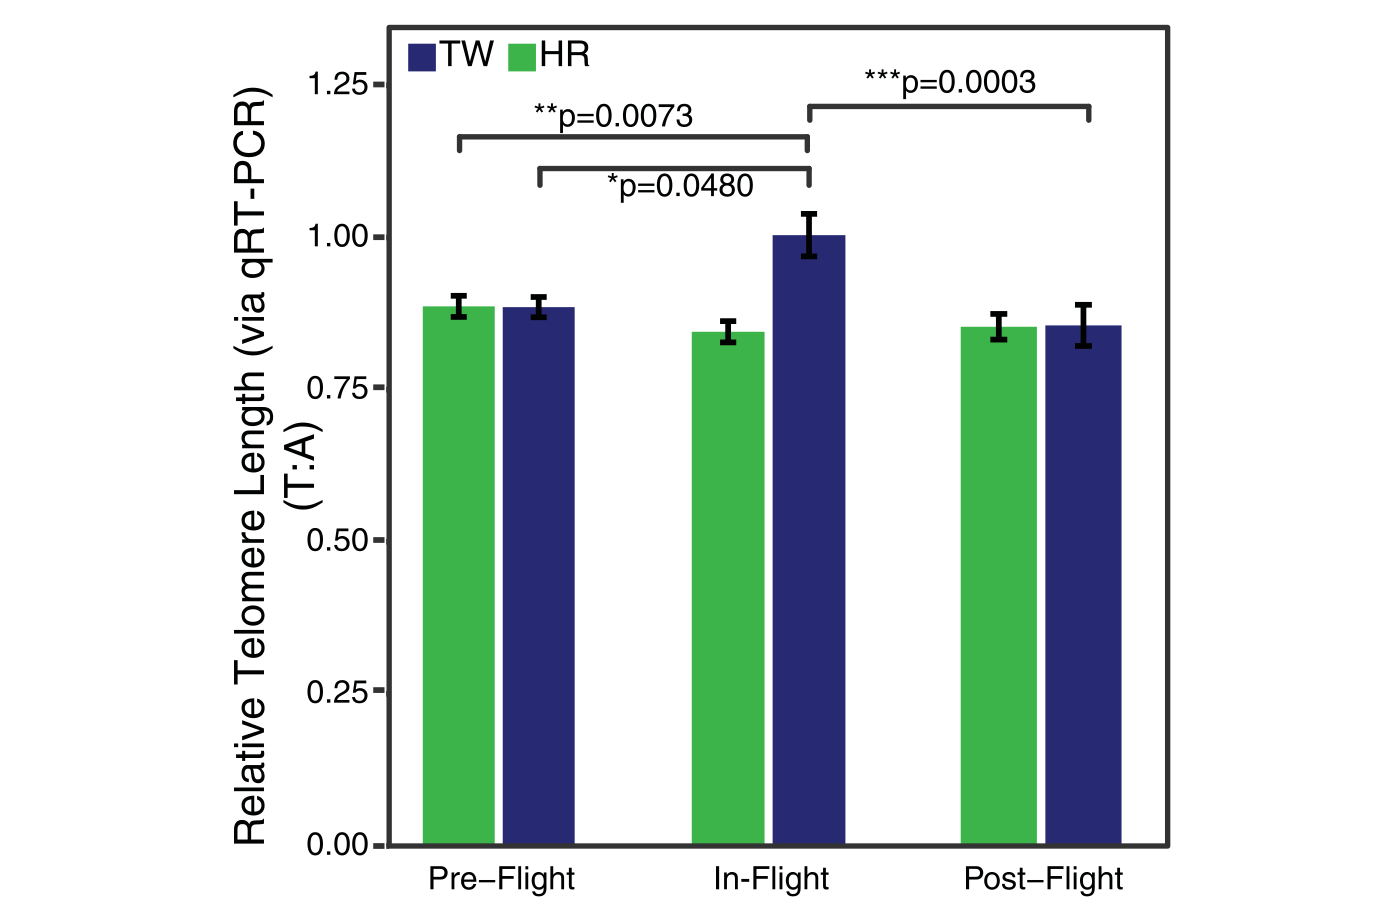
\includegraphics[width=\linewidth]{twin-telomeres-wetlab.png}
            \captionof{figure}{
                Elongation of telomeres observed \\
                during space flight in the NASA Twins Study
                \textit{[Garrett-Bakelman et al., 2019]} % 10.1126/science.aau8650
            }
    \end{center}
}


\headerbox{Methods}{name=hg38ext,span=1,column=1,below=telomere_sequencing}
{
    \begin{center}
        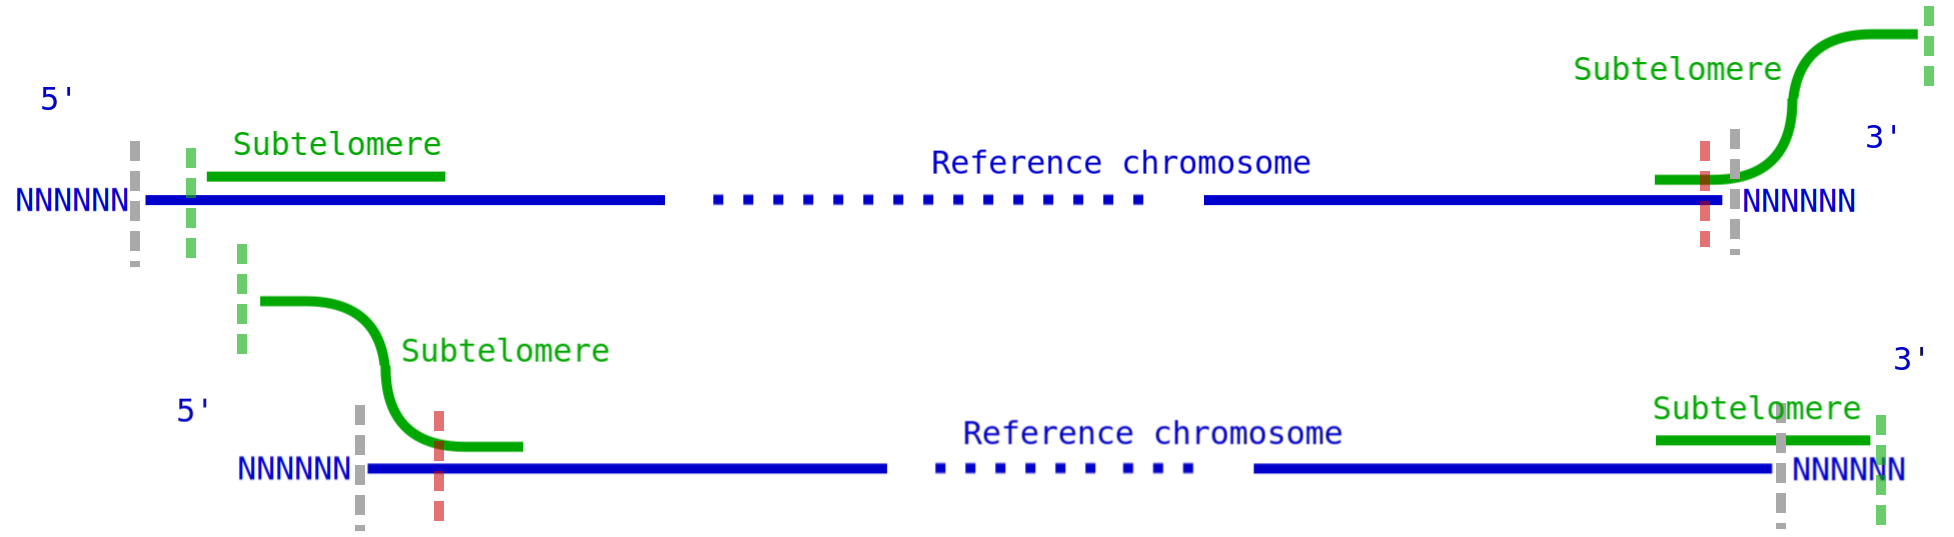
\includegraphics[width=\linewidth]{hg38ext.png}
            \captionof{figure}{
                Construction of the extended reference. Subtelomeric
                sequences were mapped to the hg38 reference and added to the
                index according to their relationship with the chromosomes. \\
                Annotated: hard-masked (unsequenced) regions (gray dashed line),
                boundaries between the subtelomere and the telomere (green),
                origins of divergent sequences (red).
            }
    \end{center}
}


\headerbox{}{name=pipeline,span=2,column=2,below=telomere_sequencing,boxheaderheight=0mm}
{
    edgeCase pipeline
}


\headerbox{Results}{name=giab_pb,span=1,column=1,below=hg38ext,boxColorOne=bluebox,headerColorOne=bluebox_adj,headerColorTwo=bluebox_adj}
{
    \begin{center}
        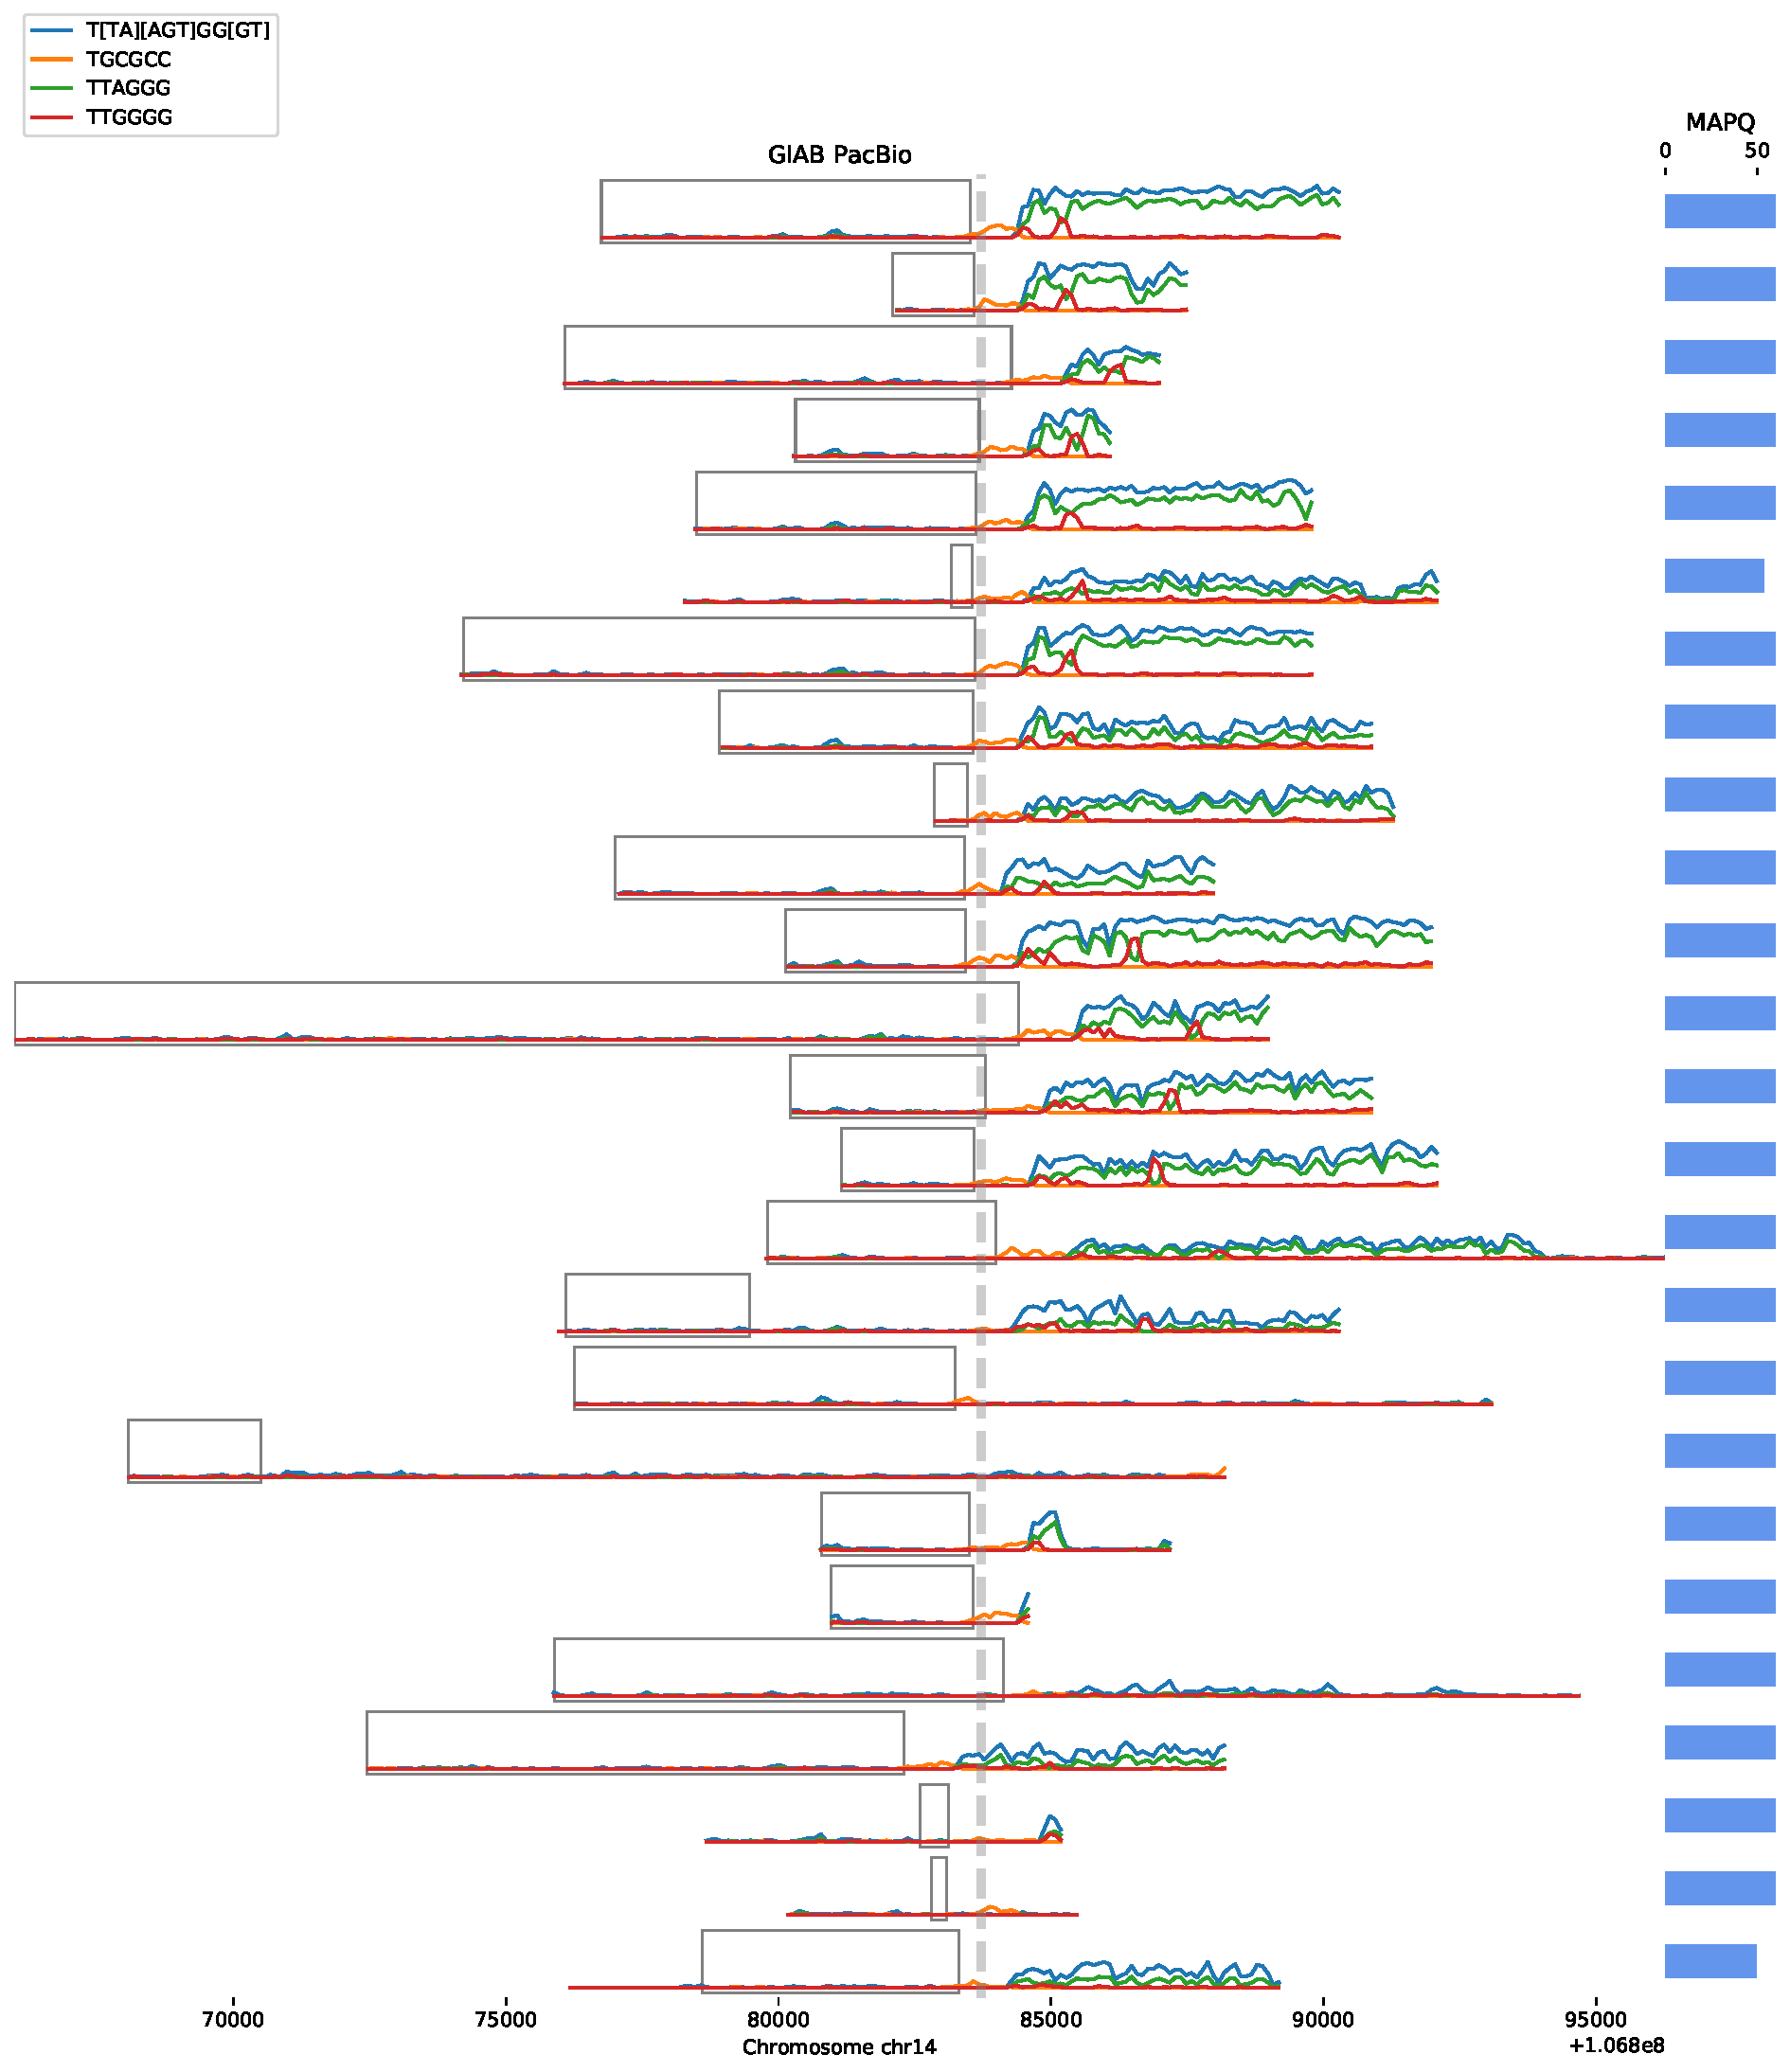
\includegraphics[width=\linewidth]{giab-pacbio-densityplot.pdf}
            \captionof{figure}{
                Distribution of major motifs in the \\ telomeric reads from the
                SMRT hg002 Genome In a Bottle
                \textit{[Zook et al., 2016]} % 10.1038/sdata.2016.25
                sample. \\
                The density plots suggest that two haplotypes are present, with
                a shorter and a longer distance between the non-canonical TTGGGG
                runs. The similarity of overall distributions suggests that the
                deviation from the canonical motif is unlikely to be due to
                random sequencing errors. \\
                Local assembly is required to describe these haplotypes.
            }
    \end{center}
}


\headerbox{}{name=no_flipflop,span=1,column=2,below=hg38ext,boxheaderheight=0mm,boxColorOne=bluebox}
{
    \begin{center}
        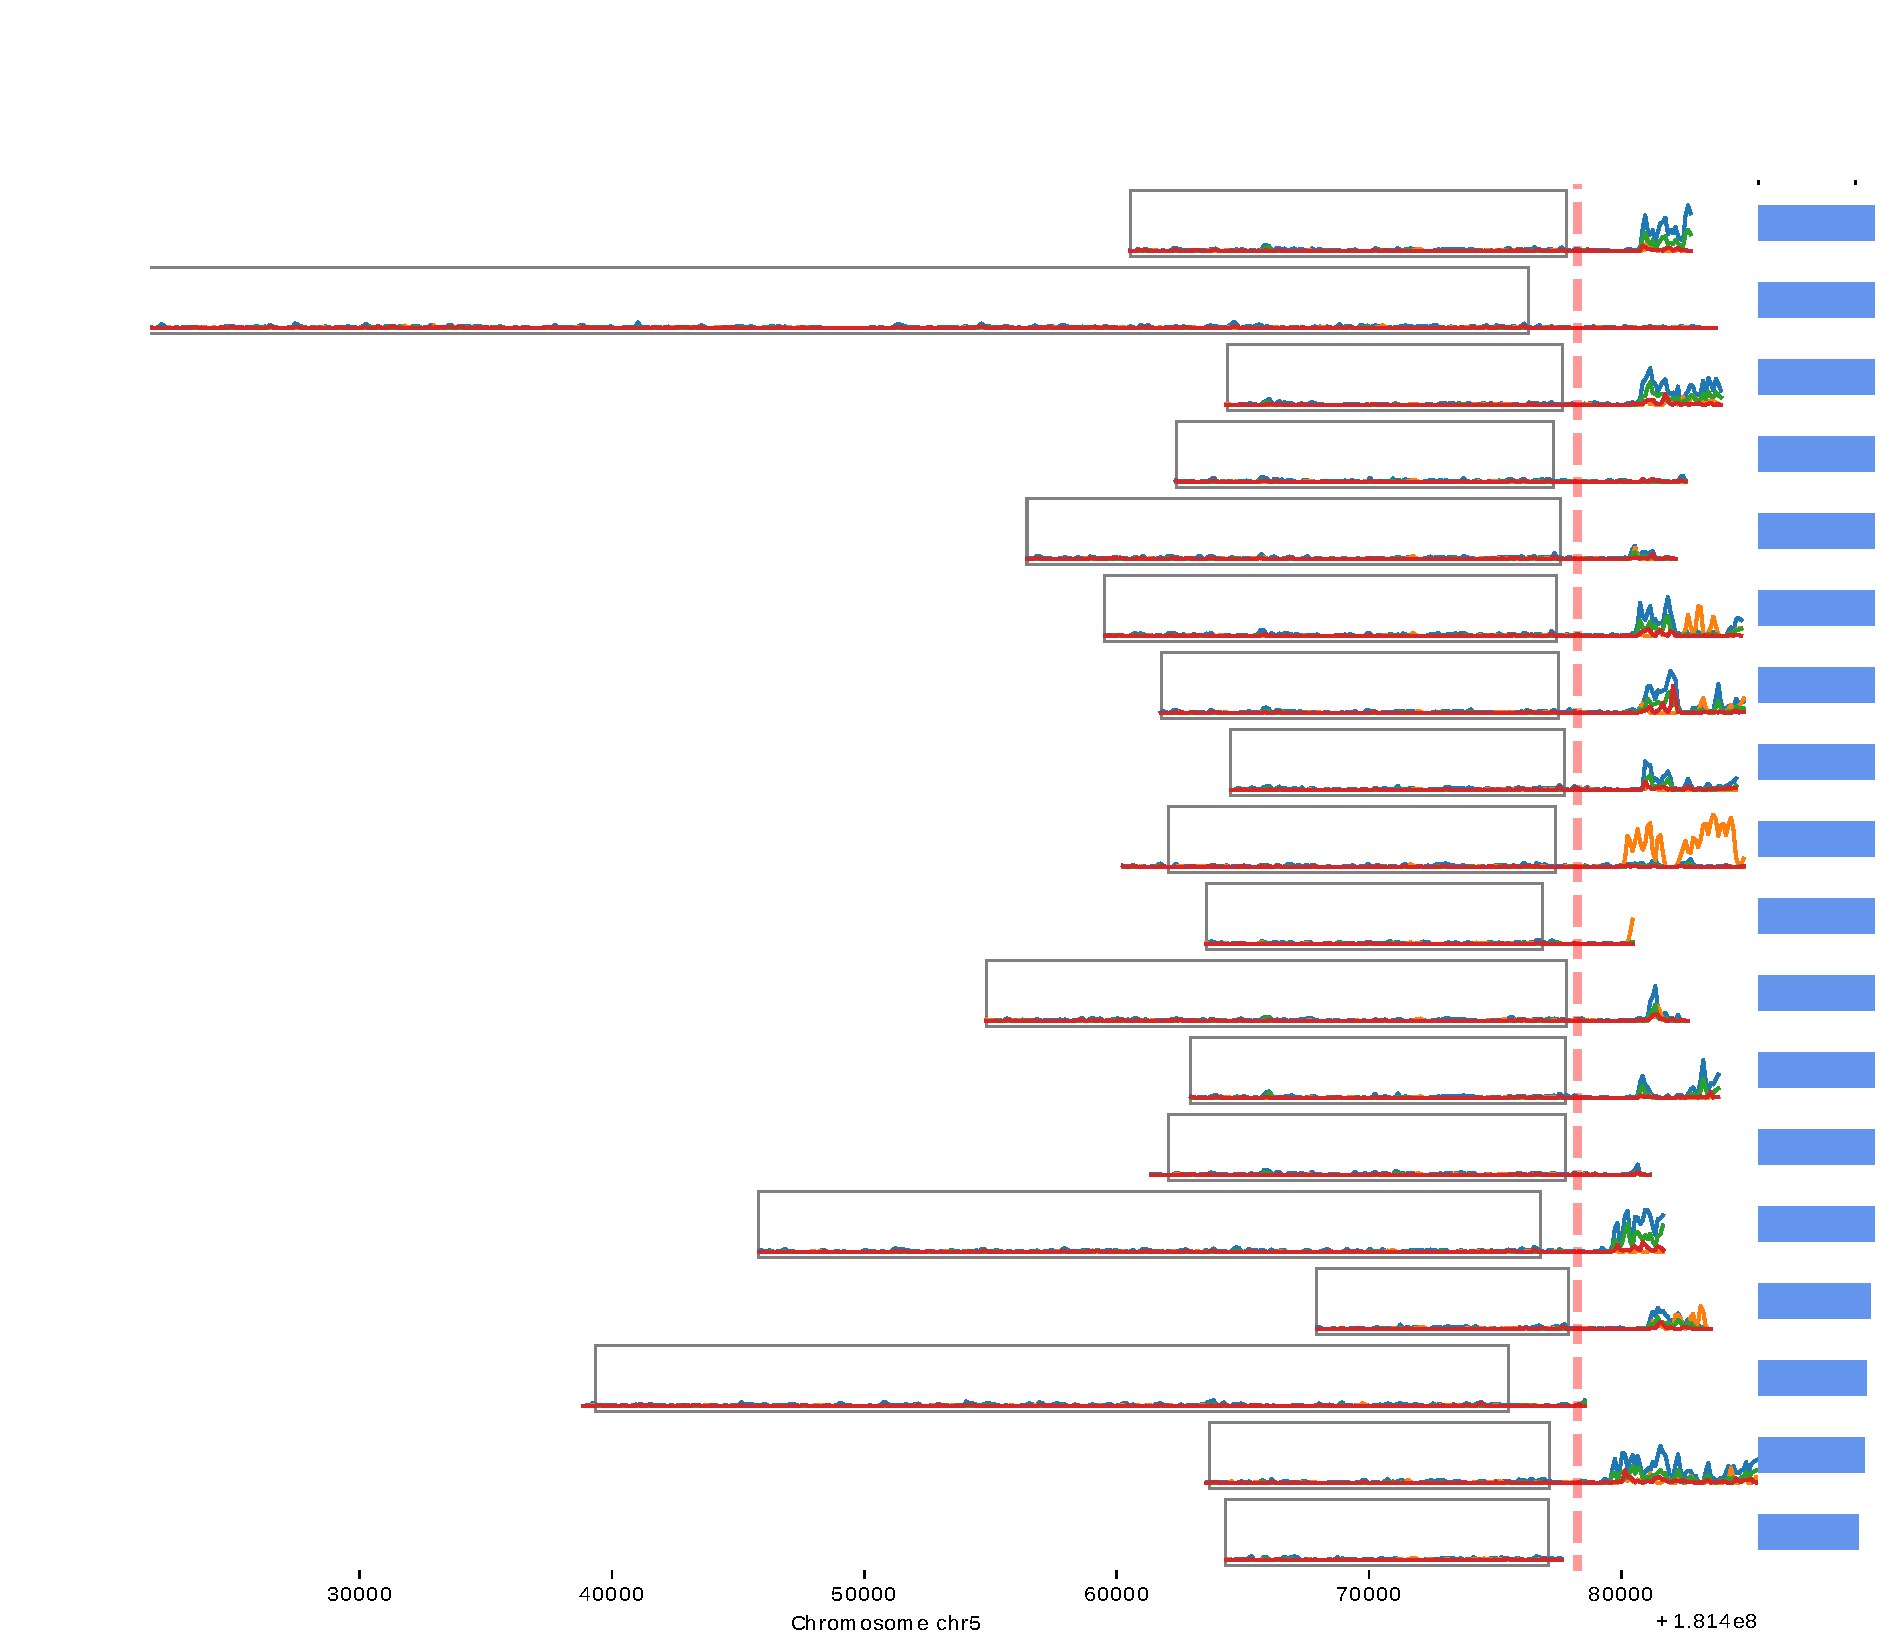
\includegraphics[width=\linewidth]{twins-noflipflop-densityplot.pdf}
            \captionof{figure}{
                Distribution of major motifs in the \\ telomeric reads from an
                internal nanopore sequencing dataset, basecalled with
                \textit{guppy} without the flip-flop model. \\
                The offending motif (orange) is GAA.
            }
    \end{center}
}


\headerbox{}{name=flipflop,span=1,column=3,below=hg38ext,boxheaderheight=0mm,boxColorOne=bluebox}
{
    \begin{center}
        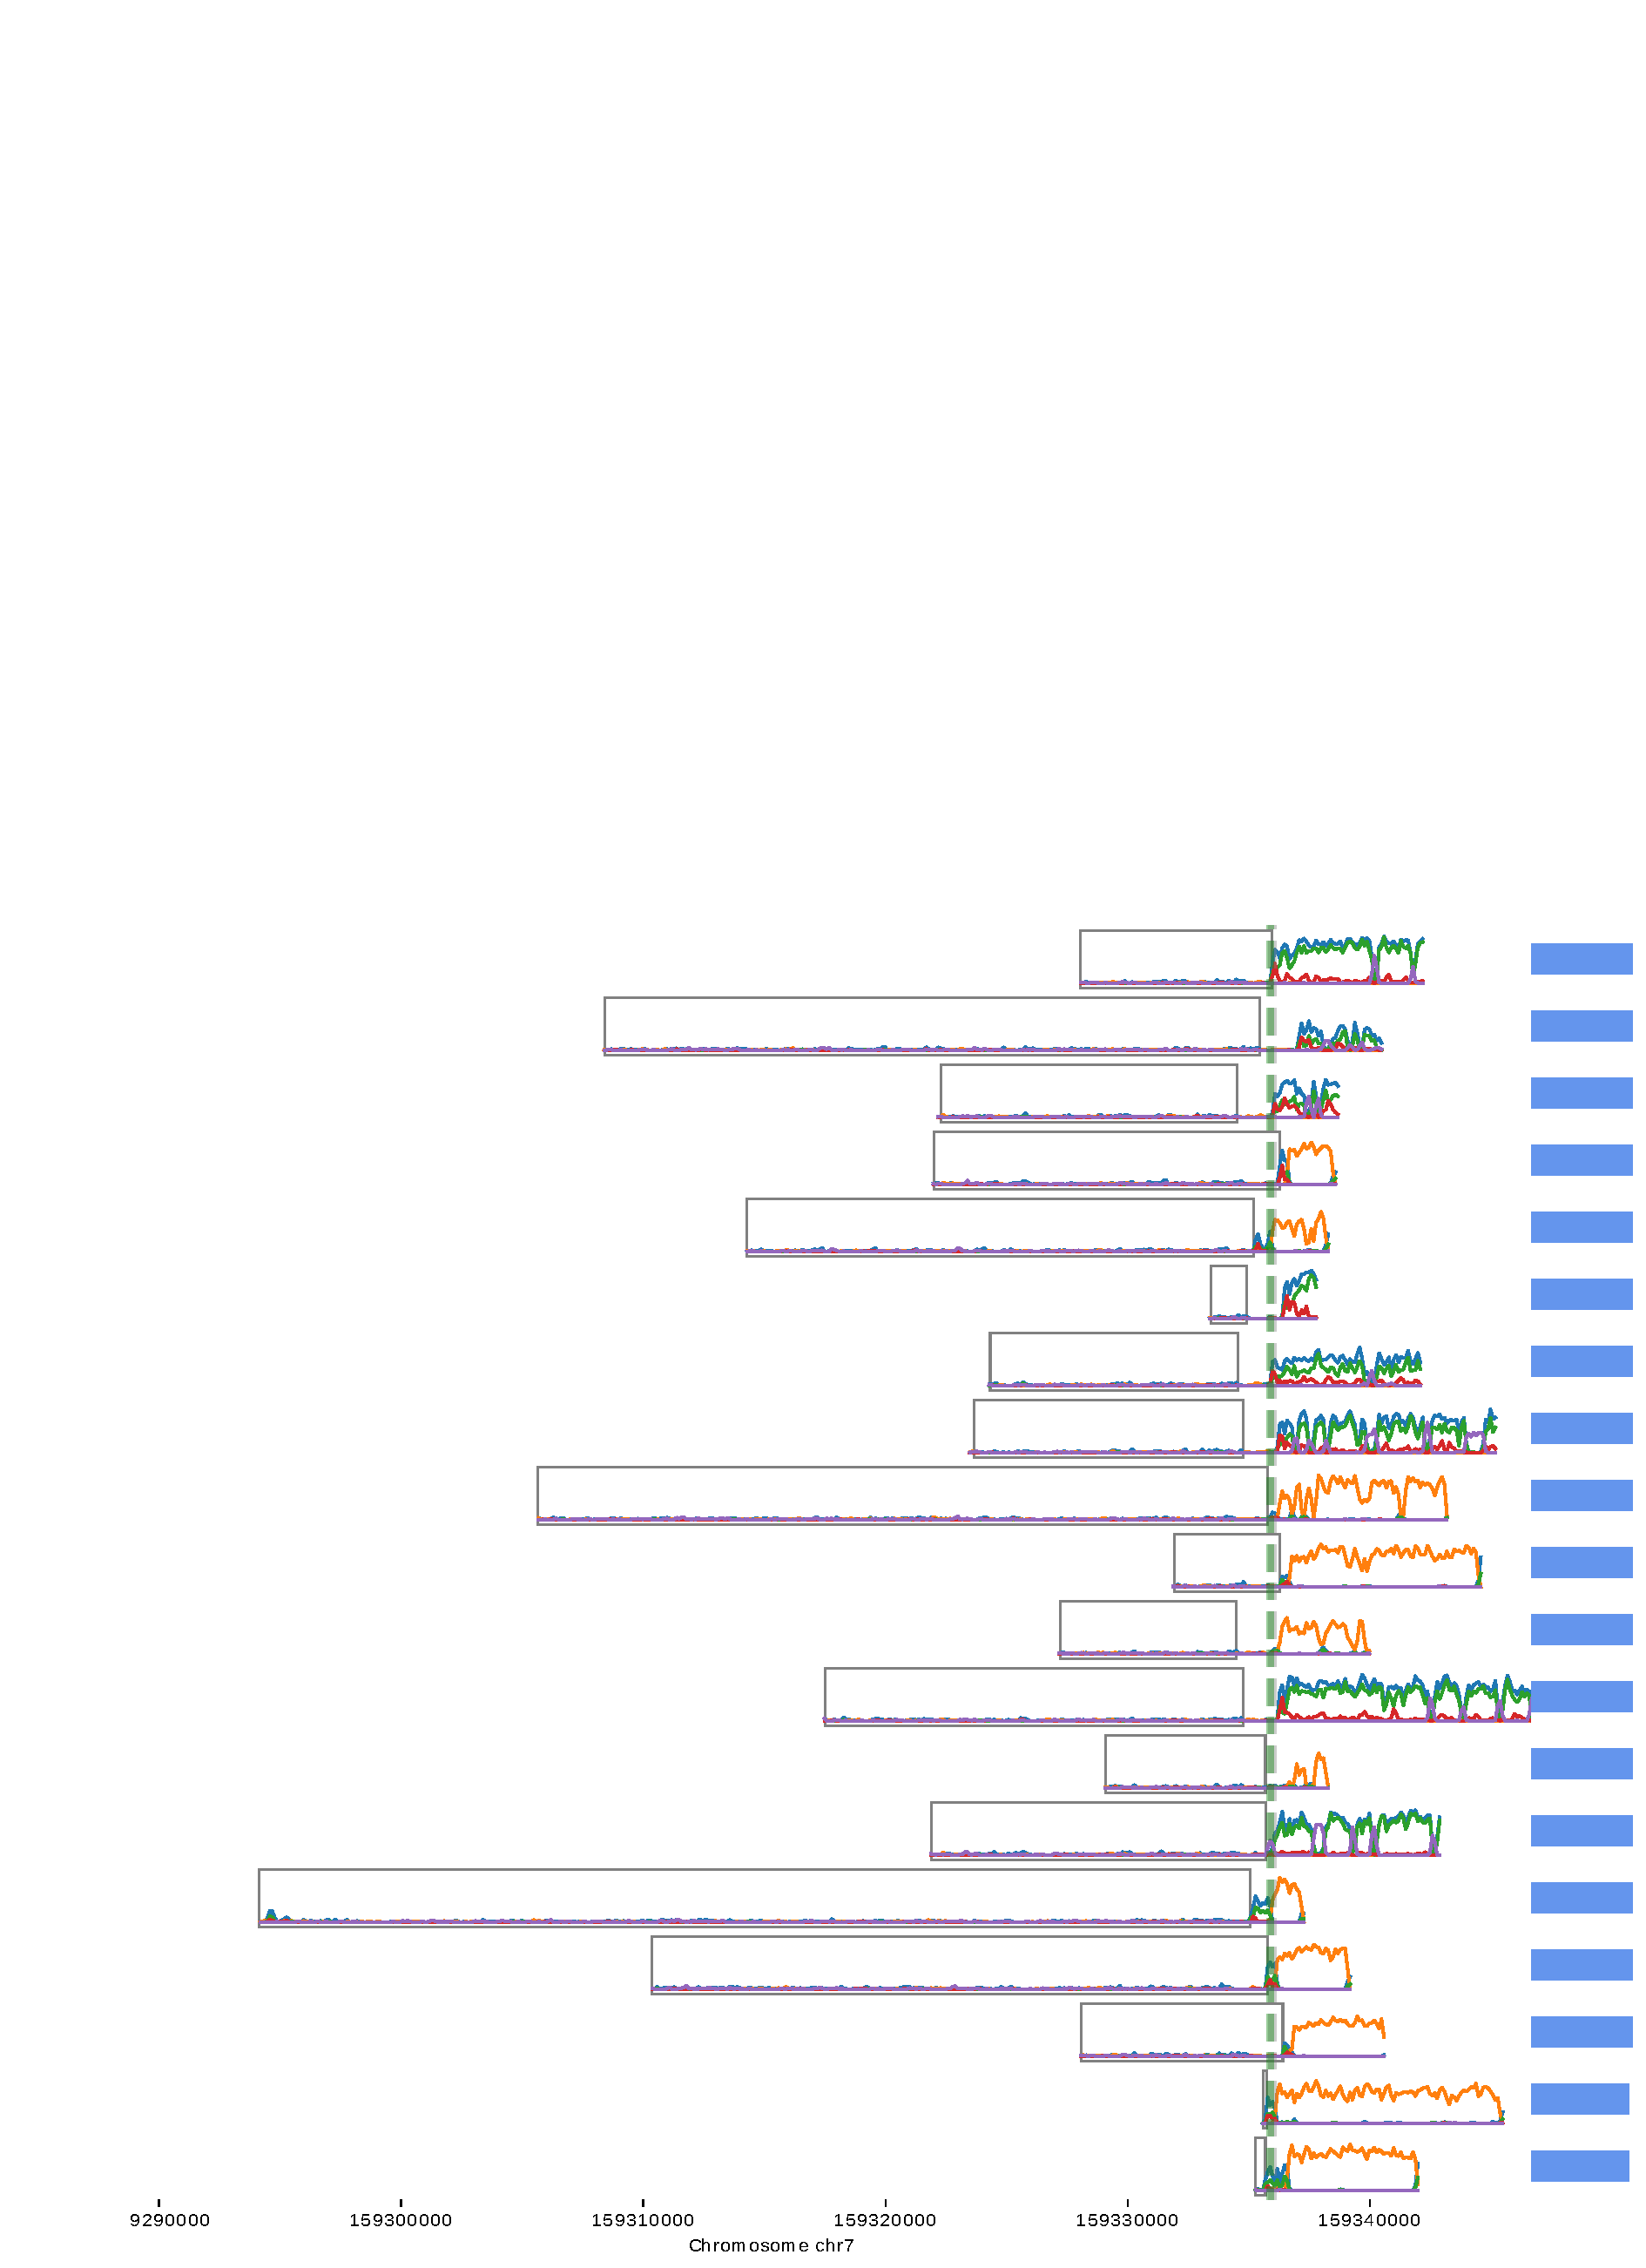
\includegraphics[width=\linewidth]{twins-flipflop-densityplot.pdf}
            \captionof{figure}{
                Distribution of major motifs in the \\ telomeric reads from an
                internal nanopore sequencing dataset, basecalled with
                \textit{guppy} \textbf{with} the flip-flop model.
                The main offending motif (orange) is CCAGG. The additional
                offending motif (purple) is TTAAAA. The same motifs are present
                in Genome In a Bottle nanopore data.
            }
    \end{center}
}


\headerbox{}{name=meme,span=1,column=1,below=giab_pb,above=bottom,boxheaderheight=0mm,boxColorOne=bluebox}
{
    \begin{center}
        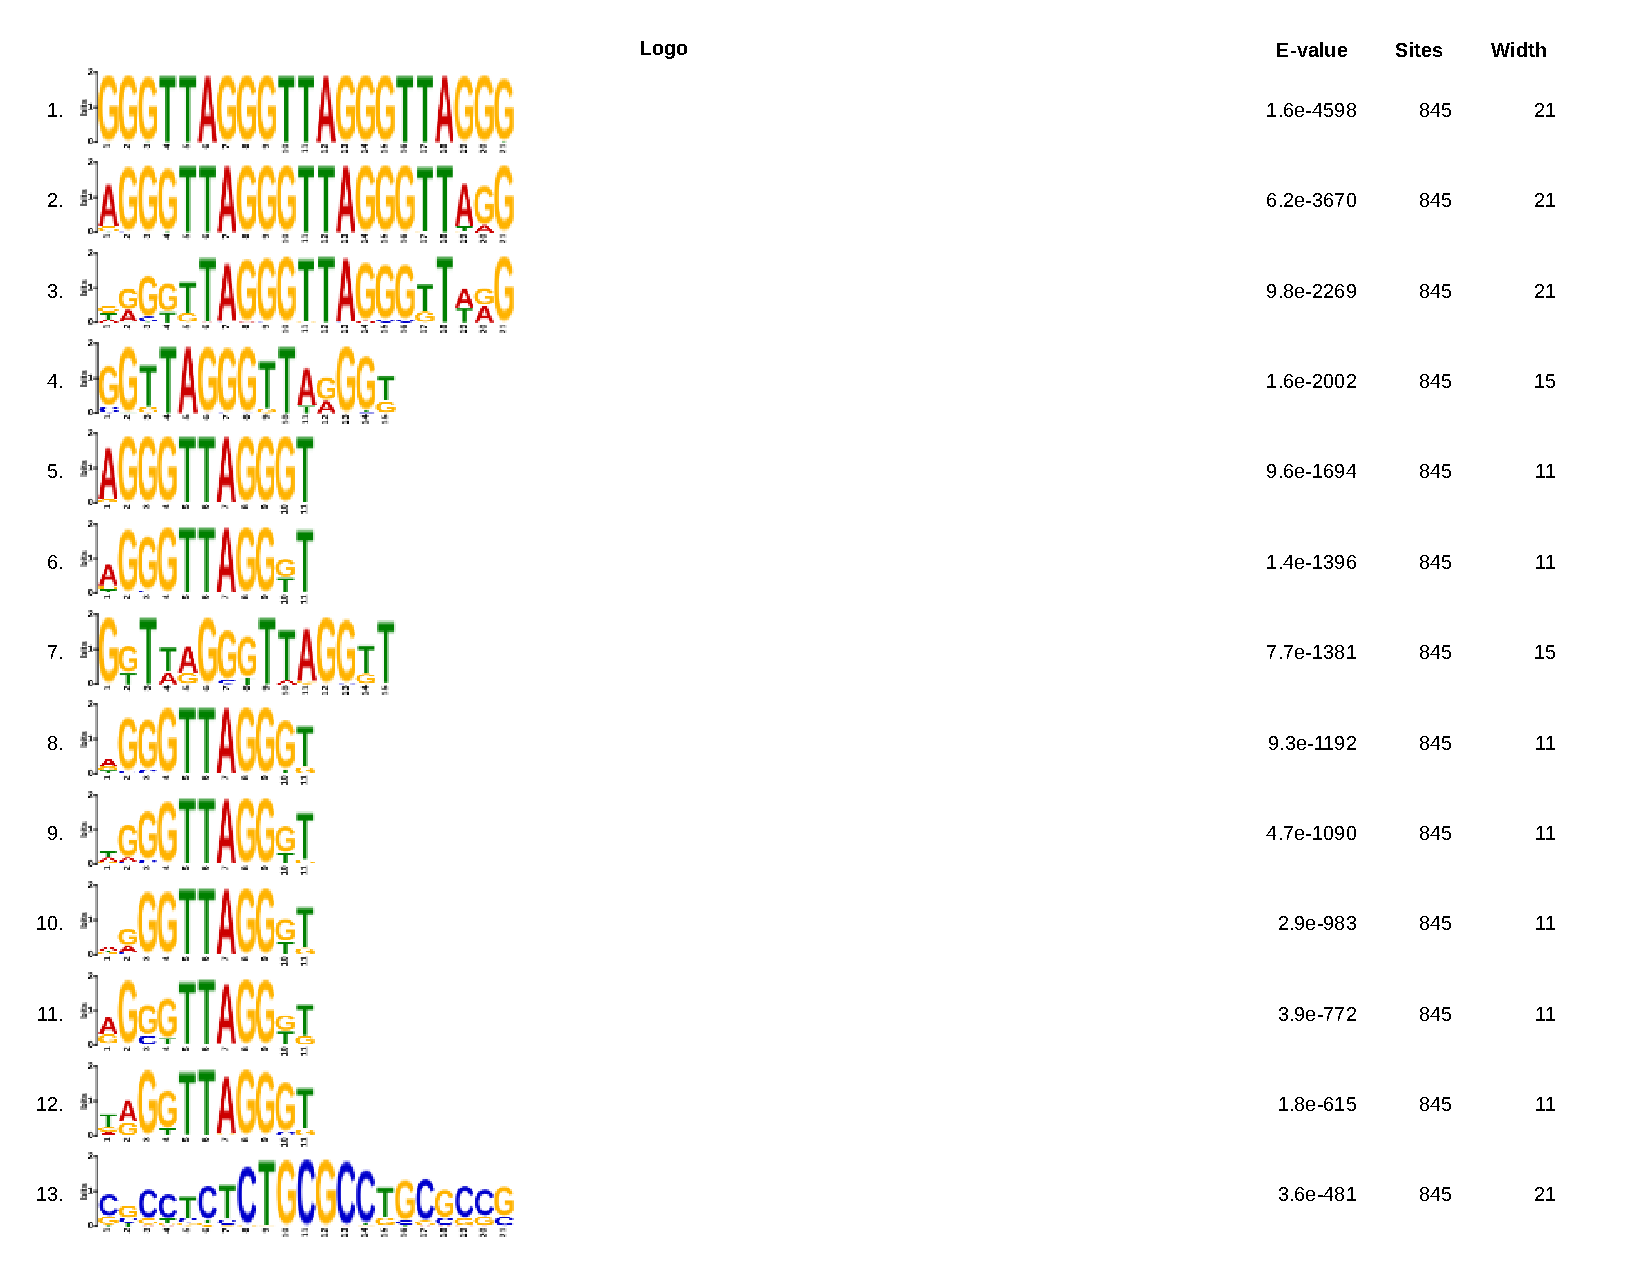
\includegraphics[width=\linewidth]{giab-pacbio-meme-top.pdf}
            \captionof{figure}{
                Motifs in segments of SMRT reads extending past the annotated
                subtelomere. \\
                Motif discovery was performed with MEME
                \textit{[Bailey et al., 1994]}
            }
    \end{center}
}


\headerbox{Further work}{name=unimizers,span=1,column=2,below=no_flipflop,above=bottom}
{
    \begin{center}
        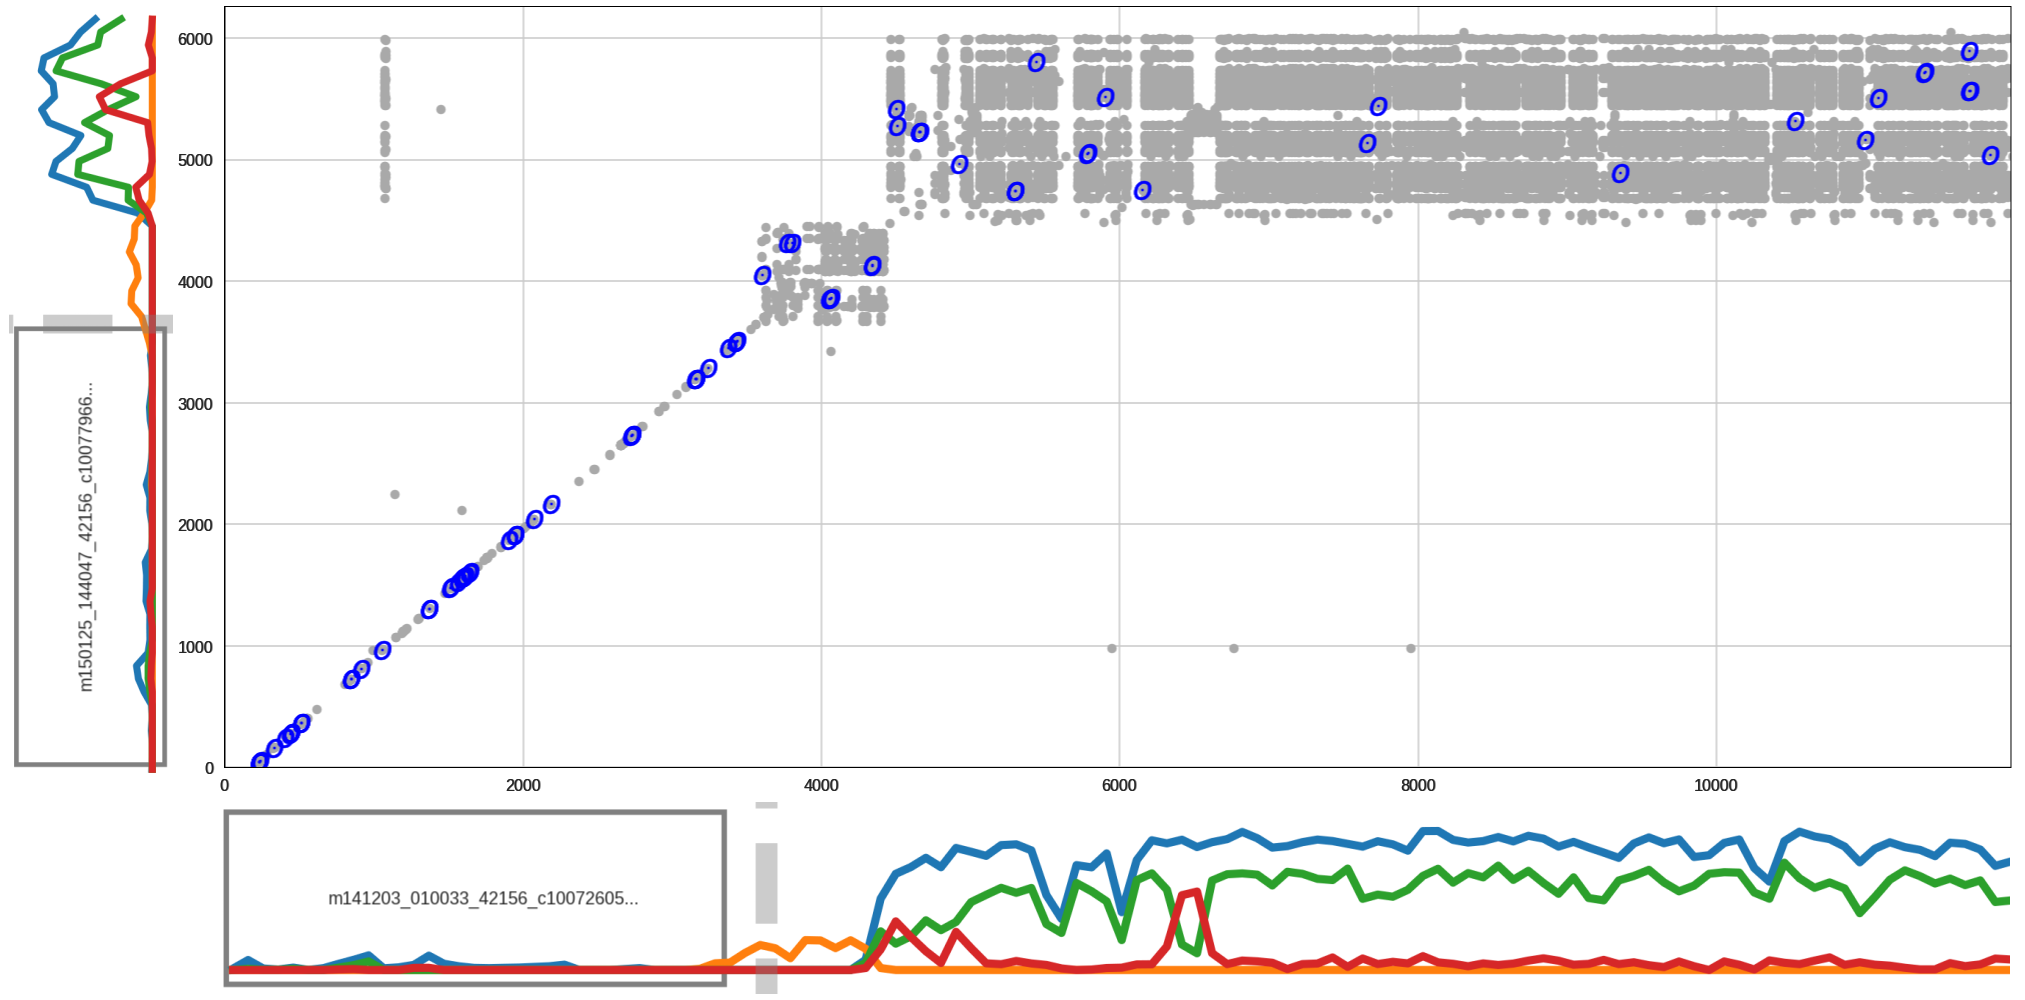
\includegraphics[width=\linewidth]{unimizers.png}
            \captionof{figure}{
                Comparison between \textit{minimizers} (gray) and
                \textit{\textbf{unimizers}} (blue), both with \textit{k}=16 and
                \textit{w}=11.
                \\
                Unimizers are minimizers that occur only once per given read.
                The same values of \textit{k} and \textit{w} in this figure are
                used for a strict comparison; more permissive values result in
                a bigger number of unimizers, especially useful for
                low-compexity regions.
                \\
                Arrays of unimizers have an advantage of
                \textit{\textbf{directionality}} compared to minimizers and
                can identify overlaps of low-complexity reads \\
                while minimizers fail to do so.
            }
    \end{center}
}


\headerbox{}{name=unimizers,span=1,column=3,below=flipflop,above=bottom,boxheaderheight=0mm}
{
    \begin{center}
        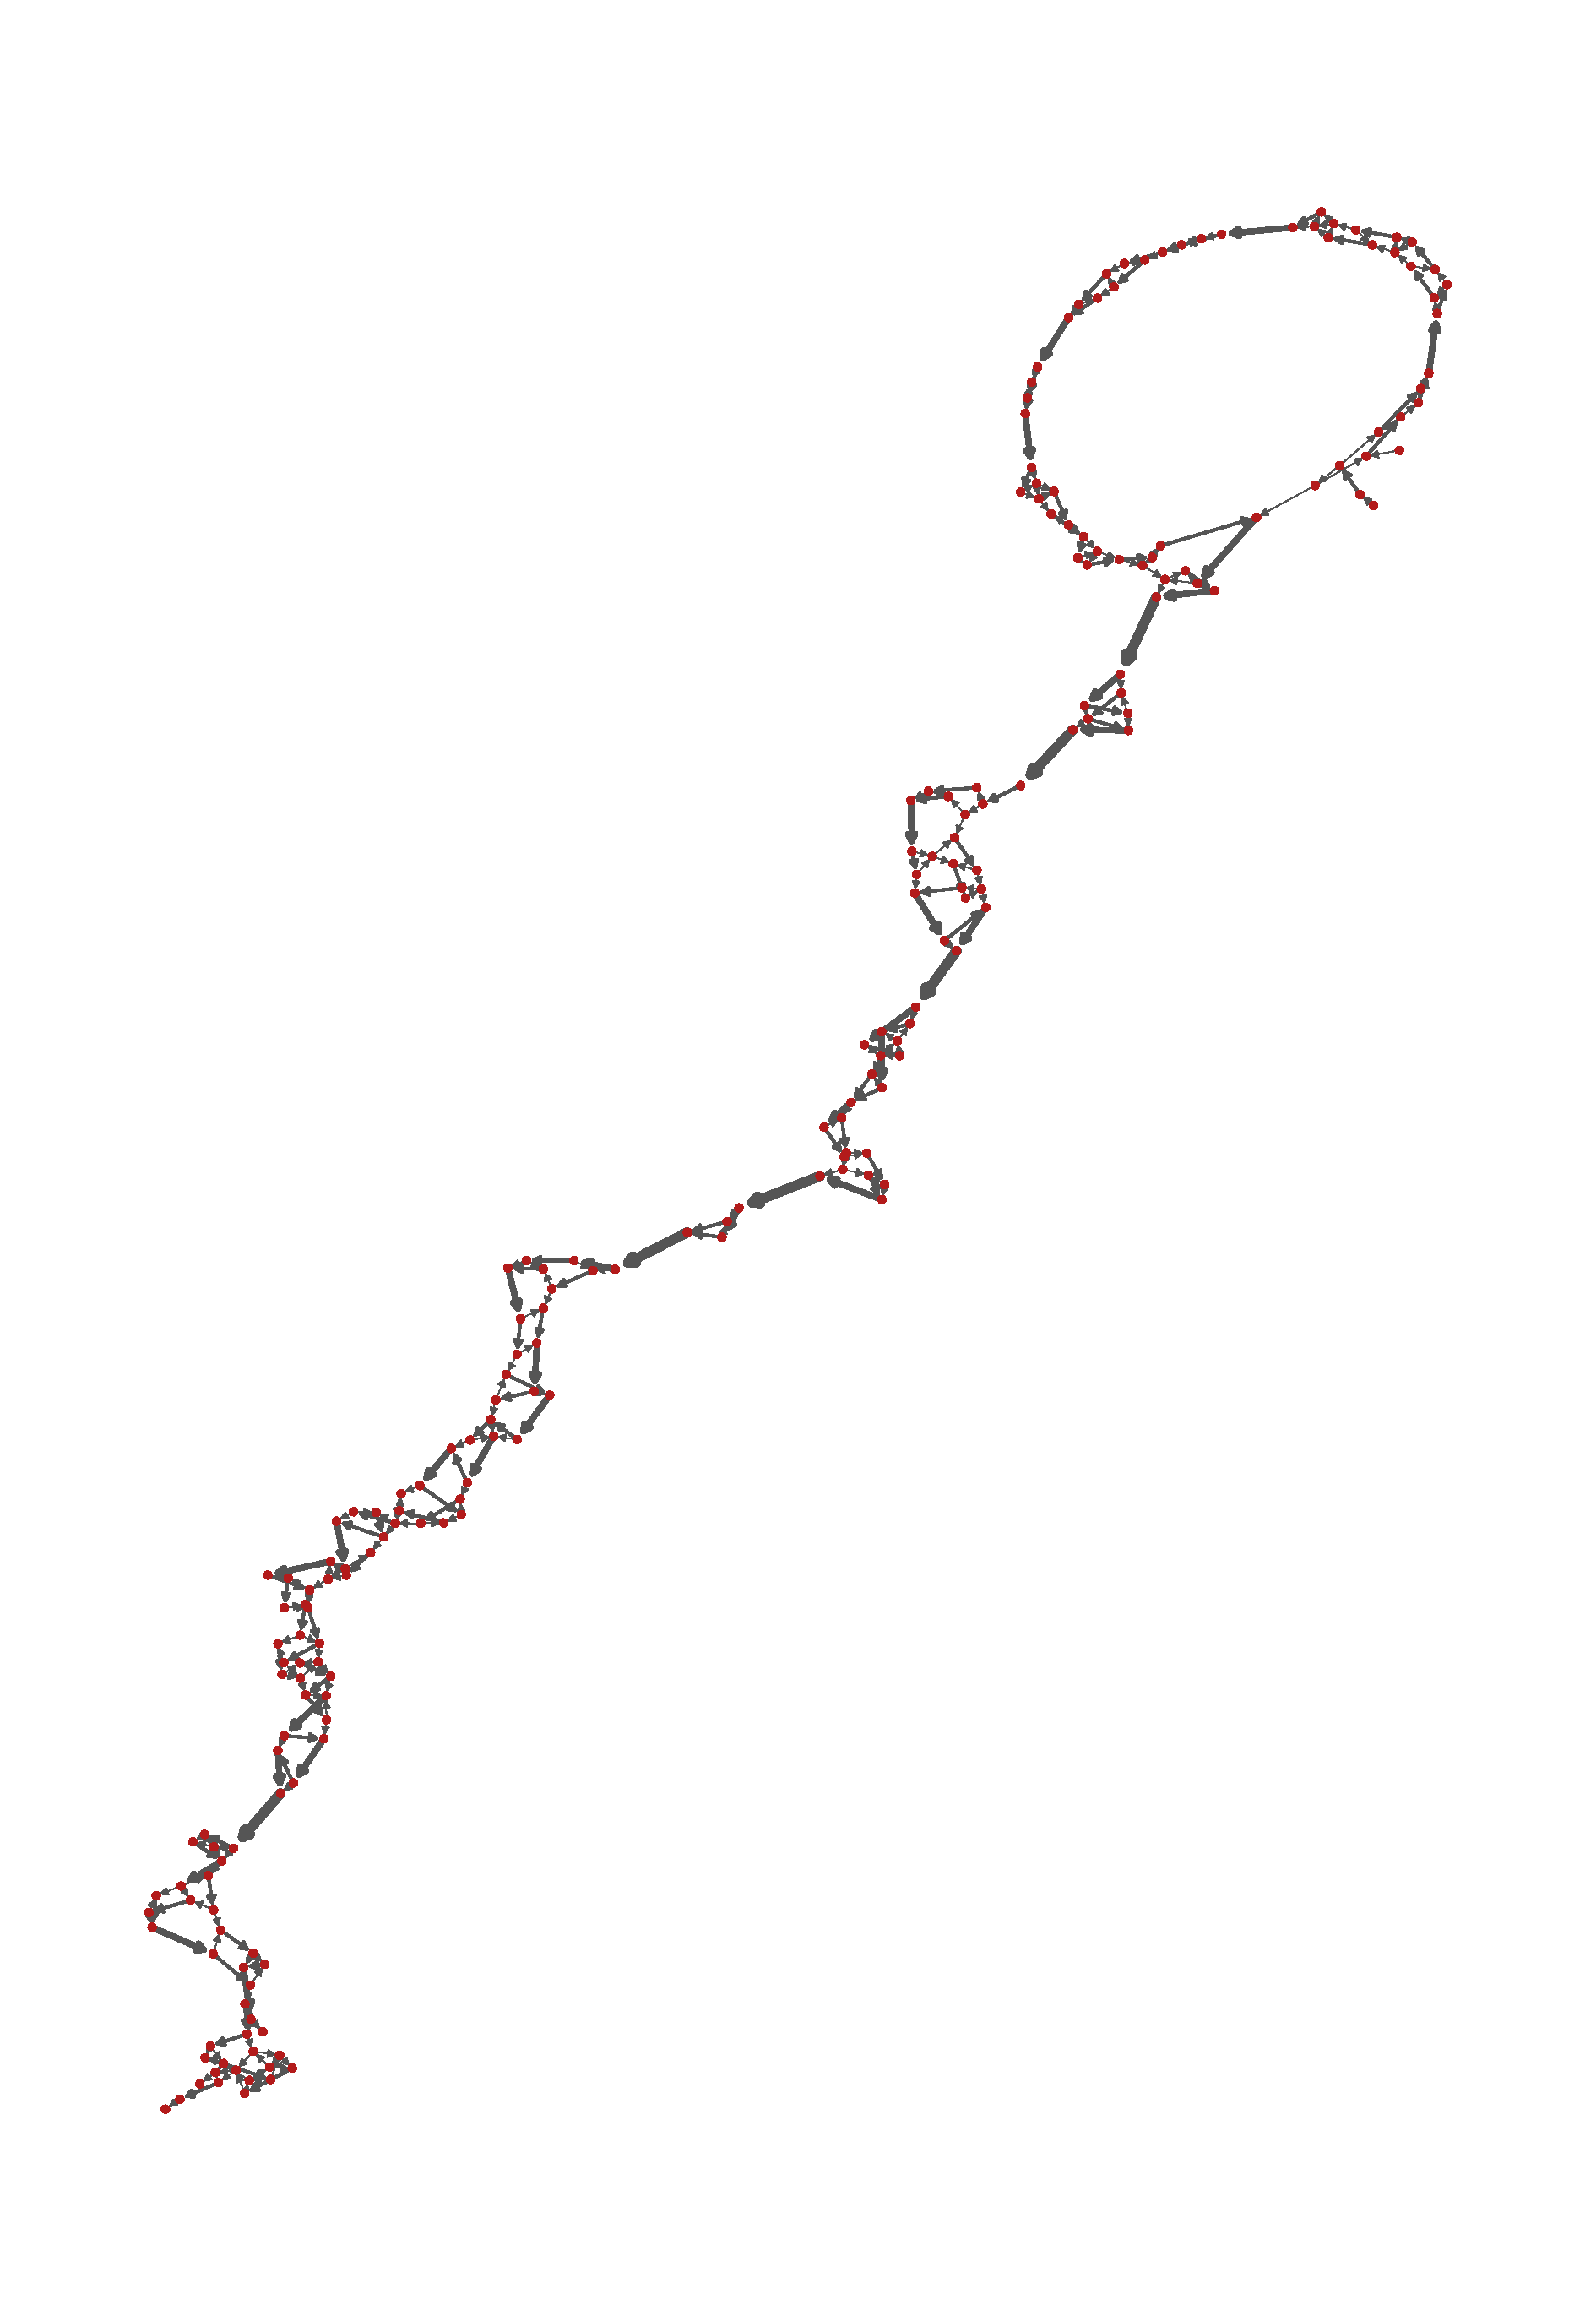
\includegraphics[angle=90,origin=c,width=\linewidth]{poster-graph.pdf}
            \captionof{figure}{
                The directionality of unimizers allows to more easily construct
                de Bruijn-like graphs (A-Bruijn graphs originally introduced in
                a different framework \textit{[Pevzner et al., 2004]}). % 10.1101/gr.2395204
        }
    \end{center}
}


\end{poster}
\end{document}
